\documentclass[11pt]{report}

% --- Language ---
\usepackage[french]{babel}
\usepackage[T1]{fontenc}
\usepackage[utf8]{inputenc}


% --- Figures ---

% Images
\usepackage{graphicx}
\graphicspath{{img/}}

% Table of contents
\usepackage[nottoc]{tocbibind}


% --- Code ---
\usepackage{minted}
\newminted{netlogo}{fontsize=\footnotesize, baselinestretch=1, breaklines, tabsize=2}
\usepackage{tcolorbox}
\usepackage{etoolbox}
\BeforeBeginEnvironment{minted}{\begin{tcolorbox}[left=0pt, right=0pt, top=0pt, bottom=0pt]}%
\AfterEndEnvironment{minted}{\end{tcolorbox}}%


% --- Layout ---
% Cover
\usepackage{titling}

% Page
\usepackage[a4paper, left=2.5cm, right=2.5cm, top=2.5cm, bottom=2.5cm]{geometry}
\usepackage{lscape}

% Font
\usepackage{libertine}

% Line spacing
\renewcommand{\baselinestretch}{1.25}
\usepackage{titlesec}
\titleformat{\chapter}{\Huge\bfseries}{\chaptername\ \thechapter}{0pt}{\vskip 20pt\raggedright}
\titlespacing{\chapter}{0pt}{20pt}{10pt}[0pt]

% Colors
\usepackage{xcolor}

\usepackage{hyperref}

% --- Drafting ---
\usepackage[chapter]{easy-todo}



\begin{document}

\begin{titlepage}
	\centering
	
\includegraphics[scale=0.8]{logo}\\
	\vspace{5cm}
	{\Huge{ \bf{Simulation Centrée Individus}}}\\
	\vspace{0.5cm}
   	{\Huge{\bf {Projet NetLogo}}}\\
	\vspace{2cm}
   	{\huge{SimCity}}\\
	\vspace{3cm}
   	{\large{Quentin Brault}}
	\vfill
	{\large Décembre 2018\par}
\end{titlepage}

\tableofcontents
\newpage

\chapter*{Introduction}
\addcontentsline{toc}{chapter}{Introduction}


Dans ce rapport sera présenté le jeu SimCity réalisé en NetLogo sur une période d'un mois et demi. La version finale reprend les éléments essentiels de la franchise, mais n'est cependant pas une copie.\\
Il aurait été intéressant d'ajouter beaucoup d'autres choses comme par exemple :
\begin{itemize}
	\item Une win/lose condition
	\item De la pollution
	\item Des déchets
	\item Des batteries
	\item Des naissances et décès
	\item Une météo
	\item Des évèvements (catastrohpes naturelles, grèves, etc...)
\end{itemize}
Mais avec près de 1600 lignes de code, dont plus de la moitié ont été réécrites au moins une fois, il était nécessaire de s'arrêter là pour rester dans le cadre du projet SCI.\\
Le projet peut être téléchargé à cette adresse :\\
\url{https://github.com/Tititesouris/SimCity}\\
\par
Après avoir présenté le jeu, nous analyserons dans ce rapport comment les différents éléments du jeu s'impactent entre eux et comment à partir de règles individuelles émergent des comportements collectifs.



\chapter{Présentation}

\section{Description}
Après avoir hérité de la fortune de vos parents qui ont tragiquement disparus ce Noël dernier dans un accident de machine à laver, vous décidez de quitter le confort de votre train train quotidien et d'acheter une parcelle de terre afin de réaliser votre rêve d'enfance : construire la plus belle ville du monde.\\
Pour cela vous devrez laisser courir votre imagination, planifier vos constructions, faire des choix difficiles parfois... Mais toujours, vous le ferez avec espoir et détermination, parce que c'est VOTRE PROJEEEET !!\\
À vous maintenant d'ériger votre ville et de la faire fleurir pour que vos habitants y vivent heureux.
\begin{center}
	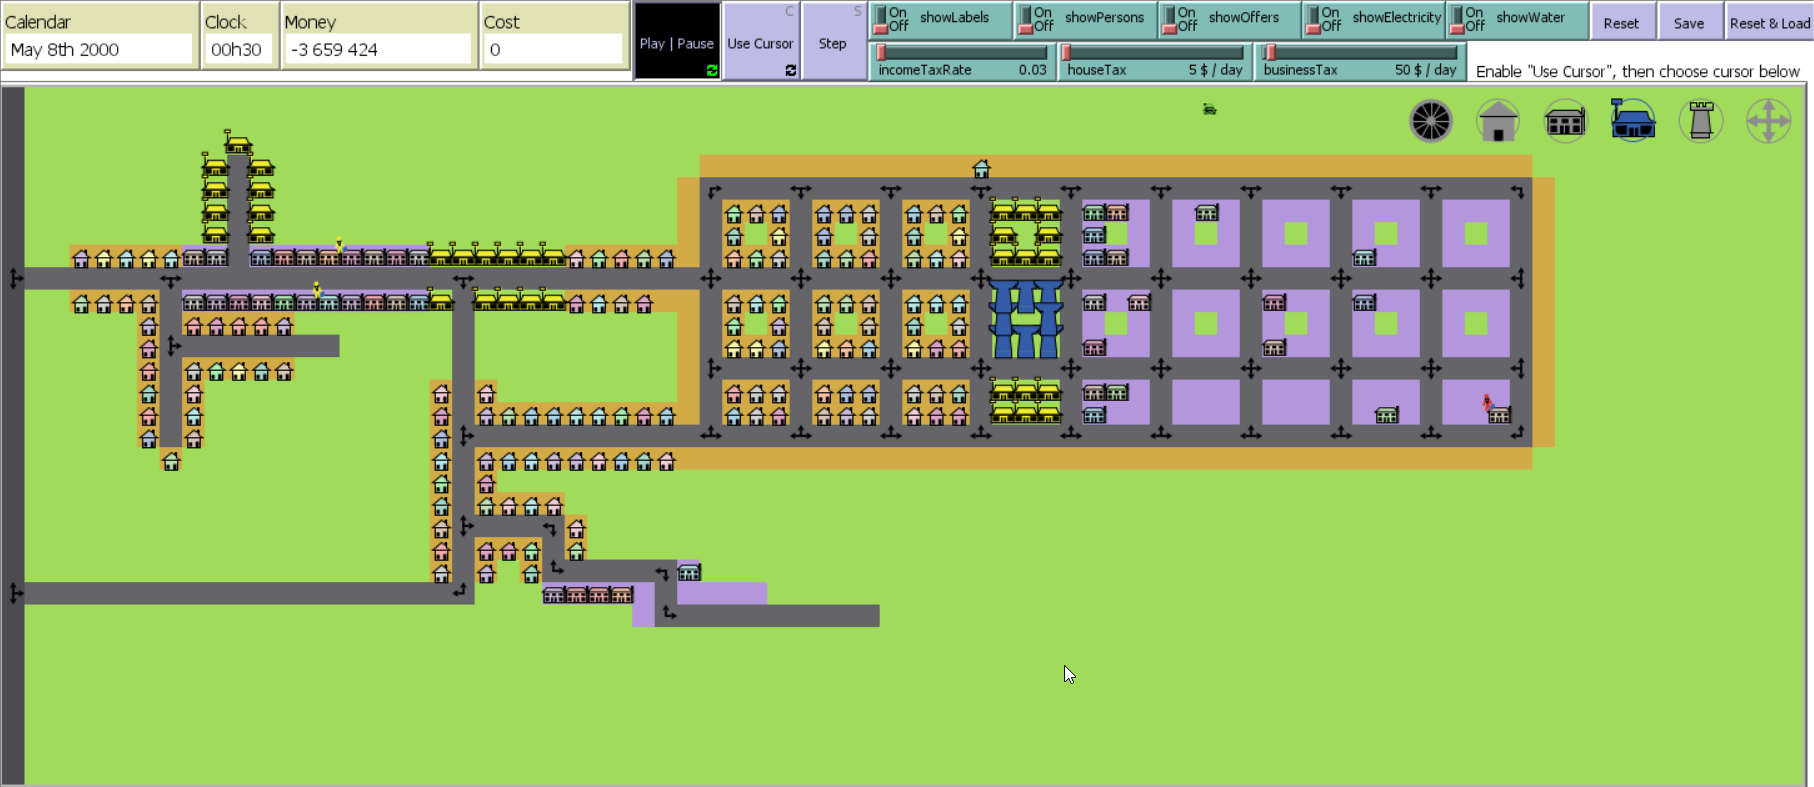
\includegraphics[width=\textwidth]{intro}
\end{center}


\newpage
\subsection{Routes}
Lorsque vous arrivez sur votre parcelle, il n'y a qu'une autoroute et un terrain vide.
L'autoroute est le seul lien entre votre ville et les villes aux alentours. C'est par cet autoroute qu'arriveront vos nouveaux habitants et que partiront vos habitants malheureux.
Pour construire un bâtiment, celui-ci doit être adjacent à une route. La première chose à faire est donc de construire une route reliée à l'autoroute afin de pouvoir commencer à construire autour.
Chaque morceau de route de votre ville vous coûte tous les jours un même coût de maintenance.\\
Les routes sont au cœur de votre ville. C'est par elles que circulent tous les agents mobiles, soit :
\begin{itemize}
	\item Les camions de déménagement qui amènent de nouveaux habitants et emmènent les habitants qui quittent votre ville.
	\item Les voitures qui conduisent vos habitants au travail et de retour chez eux.
	\item Les offres d'emploi qui permettent aux entreprises d'embaucher des habitants au chômage.
	\item Les ressources (l'électricité et l'eau) qui permettent aux bâtiments de fonctionner.
\end{itemize}


\subsection{Intersections}
\begin{center}
	\begin{minipage}{0.25\textwidth}
		\begin{flushright}
			
\includegraphics[height=80px]{intersection4}
		\end{flushright}
	\end{minipage}
	\begin{minipage}{0.7\textwidth}
		\textbf{Propriétés}
		\begin{itemize}
			\item Direction nord (Oui / Non)
			\item Direction est (Oui / Non)
			\item Direction sud (Oui / Non)
			\item Direction ouest (Oui / Non)
		\end{itemize}
	\end{minipage}
\end{center}
Lorsqu'une route que vous construisez croise une autre route, une intersection est automatiquement créée. Vous pouvez modifier ces intersections manuellement et en ajouter d'autres afin de rediriger le flot de la circulation.\\
Comme ce sont par les routes que transitent les agents mobiles, le choix des intersections impacte directement la gestion de votre ville.\\
Cependant, comme les intersections créées automatiquement vont dans toutes les directions possibles et que le concept de congestion n'existe pas, il n'est généralement pas nécessaire d'y toucher pour garantir le bon fonctionnement de votre ville.\\
\\
Il existe deux comportement d'agents mobiles aux intersections.
Le premier, le comportement aléatoire, choisit une direction au hasard, si possible pas celle d'où l'agent provient, et continue dans cette direction.
Le deuxième, le comportement de clonage, est plus complexe.\\
Dans le comportement de clonage, les agents font partie d'un groupe. Ce groupe correspond à l'ensemble des clones d'un agent. Lorsqu'un agent du groupe est modifié, tous les autres le sont aussi.\\
À chaque intersection l'agent se clone autant de fois qu'il y a de direction à cette intersection. Chaque clone est affecté au même groupe que l'agent originel. Lorsqu'un agent atteint une intersection déjà visitée, il disparaît. Le dernier agent d'un groupe à atteindre une intersection déjà visitée ne disparaît pas. Au lieu de cela, il oublie les intersections qu'il a visitées et continue son chemin, se clonant de nouveau à la prochaine intersection.



\newpage
\subsection{Agents mobiles}
\begin{center}
	
\includegraphics[height=30px]{movingtruck}
	\hspace{1cm}
	
\includegraphics[height=30px]{car}
	\hspace{1cm}
	
\includegraphics[height=30px]{offer}
	\hspace{1cm}
	
\includegraphics[height=30px]{electricity}
	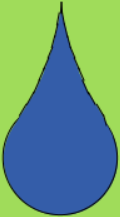
\includegraphics[height=30px]{water}
\end{center}

\subsubsection{Camions de déménagement}
Les camions de déménagement ont deux fonctions. Amener de nouveaux habitants dans votre ville et emmener des habitants qui quittent votre ville en dehors de celle-ci.\\
Dans le premier cas, les camions de déménagement apparaissent sur l'autoroute avec des passagers qui souhaitent s'installer dans votre ville. Ils roulent alors jusqu'à trouver un emplacement libre dans une zone résidentielle pour construire une maison et emménager.
Le nombre de nouveaux camions de déménagement qui arrivent chaque jour par l'autoroute dépend de l’attractivité de votre ville. L'attractivité est directement proportionnelle au bonheur total de votre ville. Avec un bonheur de 0\% il y aura 2 nouveaux camions par jour. Avec un bonheur de 100\% il y aura 2 nouveaux camions toutes les 6 heures.\\
Dans le deuxième cas, lorsque les résidents d'une maison décident de quitter votre ville, la maison est détruite et un camion de déménagement apparait, contenant les anciens résidents. Ce camion conduira jusqu'à l'autoroute où il disparaîtra. Si un camion de déménagement est encore présent un très long temps après avoir été créé, il disparait avec ses passagers.

\subsubsection{Voitures}
Les voitures transportent vos habitants sur les routes de votre ville. Les voitures sont créées dans deux cas. Le premier, quand vos habitants quittent leur maison le matin. Le deuxième, quand vos habitants quittent leur travail le soir ou si l'entreprise met la clé sous la porte alors qu'ils étaient en train de travailler. Si les voitures sont encore présentes à l'heure où les habitants vont se coucher, elles disparaissent et les habitants rentrent immédiatement chez eux.

\subsubsection{Offres d'emploi}
Les offres d'emploi sont créées tôt le matin par les entreprises qui ont des postes non pourvus. Les offres contiennent un nombre d'emplois disponibles. Elles suivent les routes avec un comportement de clonage aux intersections jusqu'à ce que des maisons avec des résidents au chômage acceptent la totalité des emplois disponibles. Si les offres sont encore présentes au moment où les habitants quittent leur maison le matin, elles disparaissent.

\subsubsection{Ressources}
Les ressources, comme les offres d'emploi, arpentent les routes avec un comportement de clonage aux intersections. L'électricité et l'eau sont les deux ressources qui existent dans votre ville.\\
Les ressources contiennent une quantité de ressource (une charge dans le cas de l'électricité, un volume dans le cas de l'eau) qui leur est donnée à leur création et qui diminue à chaque fois qu'un bâtiment en consomme une part. Si les ressources sont encore présentes quelques heures après avoir été créées, elles disparaissent. Les ressources sont utilisées par différents bâtiments. Ces bâtiments stockent une partie des ressources pour pouvoir les consommer en attendant d'en recevoir plus.



\newpage
\subsection{Maisons}
\begin{center}
	\begin{minipage}{0.25\textwidth}
		\begin{flushright}
			
\includegraphics[height=45px]{house_beige}
			
\includegraphics[height=45px]{house_green}\\
			
\includegraphics[height=45px]{house_blue}
			
\includegraphics[height=45px]{house_pink}
		\end{flushright}
	\end{minipage}
	\begin{minipage}{0.7\textwidth}
		\textbf{Propriétés}
		\begin{itemize}
			\item Consommation d'électricité (kWh)
			\item Consommation d'eau (L/h)
			\item Bonheur (\%)
			\item Nombre de chambres
			\item Résidents
		\end{itemize}
	\end{minipage}
\end{center}

Une maison se construit automatiquement sur une case libre de zone résidentielle lorsqu'un camion de déménagement passe à proximité. Les passagers du camion de déménagement s'installent alors dans la maison et le camion disparaît.\\
Chaque maison a un besoin d'eau et d'électricité qui dépend du nombre de résidents et du nombre de résidents à la maison. Une maison sans résident est automatiquement détruite.\\
Les maisons de votre ville vous payent, chacune, tous les jours, un même impôt dont vous pouvez ajuster le montant.
Le bonheur d'une maison est calculé tous les ticks en fonction des avertissements sur cette maison de la manière suivante :\\
Le bonheur commence à 100\%. Pour chaque avertissement, le bonheur et diminué de 10 fois l'importance de l'avertissement. Le bonheur ne peut pas descendre en dessous de 0\%.
Avec un avertissement de manque d'eau d'importance 1 et un avertissement d'impôts trop élevés d'importance 2, le bonheur est donc de $100 - 10 * (1 + 2) = 70\%$.\\
Si le bonheur descend en dessous de 50\%, il y a une probabilité que tous les habitants de la maison déménagent. Plus le bonheur est bas, plus cette probabilité augmente jusqu'à atteindre 100\%/


\subsection{Entreprises}
\begin{center}
	\begin{minipage}{0.35\textwidth}
		\begin{flushright}
			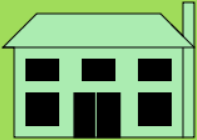
\includegraphics[width=65px]{business_green}
			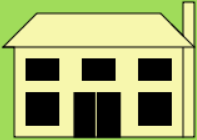
\includegraphics[width=65px]{business_yellow}\\
			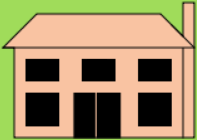
\includegraphics[width=65px]{business_beige}
			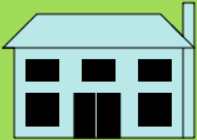
\includegraphics[width=65px]{business_blue}
		\end{flushright}
	\end{minipage}
	\begin{minipage}{0.6\textwidth}
		\textbf{Propriétés}
		\begin{itemize}
			\item Consommation d'électricité (kWh)
			\item Consommation d'eau (L/h)
			\item Bonheur (\%)
			\item Nombre d'emplois
			\item Salariés
		\end{itemize}
	\end{minipage}
\end{center}

Une entreprise se construit automatiquement sur une case libre de zone d'activités économiques lorsqu'une voiture avec un passager chômeur passe à proximité. Les passagers chômeurs viennent en effet de créer leur entreprise et en deviennent les premiers salariés.\\
Chaque entreprise a un besoin d'eau et d'électricité qui dépend du nombre de salariés et du nombre de salariés à la maison.
Les entreprises de votre ville vous payent, chacune, tous les jours, un même impôt dont vous pouvez ajuster le montant.\\
De la même manière que pour les maisons, le bonheur d'une entreprise est calculé tous les ticks en fonction des avertissements sur cette entreprise :\\
Le bonheur commence à 100\%. Pour chaque avertissement, le bonheur et diminué de 10 fois l'importance de l'avertissement. Le bonheur ne peut pas descendre en dessous de 0\%.
Si le bonheur descend en dessous de 50\%, il y a une probabilité que l'entreprise ferme. Plus le bonheur est bas, plus cette probabilité augmente jusqu'à atteindre 100\% de chance.


\subsection{Personnes}
\begin{center}
	\begin{minipage}{0.6\textwidth}
		\begin{flushright}
			
\includegraphics[height=100px]{person_0}
			
\includegraphics[height=100px]{person_1}
			
\includegraphics[height=100px]{person_2}
			
\includegraphics[height=100px]{person_3}
		\end{flushright}
	\end{minipage}
	\begin{minipage}{0.35\textwidth}
		\textbf{Propriétés}
		\begin{itemize}
			\item Résidence
			\item Employeur
			\item Bonheur (\%)
			\item Salaire (\$/jour)
		\end{itemize}
	\end{minipage}
\end{center}

Les personnes qui ont une résidence sont les habitants de votre ville. Les personnes sans résidence sont soit en train d'emménager soit en train de quitter votre ville.
Vos habitants sont au chômage jusqu'à ce qu'ils trouvent un employeur par le biais d'une offre d'emploi ou bien qu'ils créent leur propre entreprise.
Tous les habitants quittent leur maison dans la matinée et montent dans leurs voitures. S'ils ont un employeur, ils conduisent dans leur voiture jusqu'à trouver leur entreprise. S'ils sont au chômage, ils conduisent jusqu'à trouver un emplacement vide dans une zone d'activités économiques pour y fonder une entreprise.\\
Les habitants qui ont un emploi commencent avec un salaire de base qui est le même pour tous. Puis, leur salaire augmente chaque semaine de manière linéaire jusqu'à atteindre le salaire maximum (le même pour tout le monde) au bout d'un an.\\
Le bonheur d'une personne est calculé tous les ticks en fonction de sa situation d'embauche et de son salaire de la manière suivante :\\
Si la personne est au chômage, son bonheur est équivalent à 75\%, moins 1\% pour chaque 3 heures au chômage.
Si la personne est employée, son bonheur est équivalent à 50\%, plus la moitié du pourcentage du salaire de la personne par rapport au salaire maximal, moins le pourcentage d'impôts sur le revenu.
Avec un emploi, un salaire de 10\$, un salaire maximum de 100\$ et un impôt sur le revenu de 3\%, le bonheur calculé est de $50 + (10 / 100) * 50 - 3 = 52\%$.\\
Le bonheur d'un chômeur depuis 30 heures est de $75 - (30 / 3) = 65\%$.
On voit donc qu'il est tout à fait possible qu'un chômeur soit plus heureux qu'une personne avec un travail, et qu'au moment de son embauche une personne devienne plus malheureuse.\\
Si le bonheur descend en dessous de 30\%, il y a une probabilité que la personne quitte la ville. Plus le bonheur est bas, plus cette probabilité augmente jusqu'à atteindre 100\% de chance à 0\% de bonheur.



\newpage
\subsection{Zones}
\begin{center}
	\begin{minipage}{0.6\textwidth}
		Vous pouvez placer des zones autour des routes de votre ville. Ces zones indiquent quelles structures peuvent apparaître dans les emplacements de la zone. Les zones résidentielles sont indiquées en orange et les zones d'activités économiques en violet.
	\end{minipage}
	\begin{minipage}{0.35\textwidth}
		\begin{flushright}
			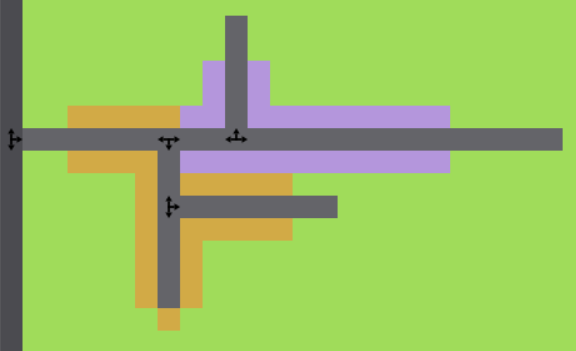
\includegraphics[height=90px]{zones}
		\end{flushright}
	\end{minipage}
\end{center}

\subsubsection{Zones résidentielles}
Les zones résidentielles indiquent un ensemble d'emplacements où de nouveaux habitants peuvent venir construire leur maison pour y habiter. Si une partie d'une zone résidentielle est remplacée par une autre zone alors touts les habitants des maisons qui s'y trouvaient déménagent de votre ville et les maisons sont détruites.

\subsubsection{Zones d'activités économiques}
Les zones d'activités économiques indiquent un ensemble d'emplacements où de nouvelles entreprises peuvent s'installer. Si une partie d'une zone d'activités économiques est remplacée par une autre zone alors toutes les entreprises qui s'y trouvaient sont détruites et les salariés renvoyés chez eux sans emploi.


\subsection{Centrales électriques}
\begin{center}
	\begin{minipage}{0.25\textwidth}
		\begin{flushright}
			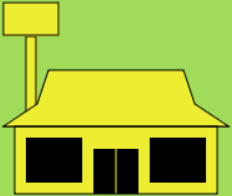
\includegraphics[height=40px]{powerplant}
		\end{flushright}
	\end{minipage}
	\begin{minipage}{0.7\textwidth}
		\textbf{Propriétés}
		\begin{itemize}
			\item Production d'électricité (kWh)
		\end{itemize}
	\end{minipage}
\end{center}
Les centrales électriques alimentent votre ville en électricité.
Elles produisent une particule d'électricité toutes les heures. La charge électrique de cette particule correspond à la production de la centrale.\\
Les centrales électriques de votre ville vous coûtent, chacune, tous les jours, un même coût de maintenance afin d'assurer leur fonctionnement.


\subsection{Pompes à eau}
\begin{center}
	\begin{minipage}{0.25\textwidth}
		\begin{flushright}
			
\includegraphics[height=45px]{pump}
		\end{flushright}
	\end{minipage}
	\begin{minipage}{0.7\textwidth}
		\textbf{Propriétés}
		\begin{itemize}
			\item Consommation d'électricité (kWh)
			\item Production d'eau (L/h)
		\end{itemize}
	\end{minipage}
\end{center}
Les pompes à eau alimentent votre ville en eau.
Elles ont besoin d'électricité pour fournir de l'eau. La quantité d'électricité nécessaire dépend de la quantité d'eau à fournir. Lorsqu'une pompe à eau reçoit suffisamment d'électricité, elle produit une particule d'eau toutes les heures. La quantité d'eau de cette particule correspond à la production de la pompe à eau.\\
Les pompes à eau de votre ville vous coûtent, chacune, tous les jours, un même coût de maintenance afin d'assurer leur fonctionnement.



\newpage
\subsection{Avertissements}
Les avertissements sont des indicateurs vous permettant de remarquer rapidement un problème dans votre ville. Ils participent également au calcul du bonheur des maisons et des entreprises.\\
\\
\begin{minipage}{0.7\textwidth}
	Les bâtiments ayant des besoins, ils affichent des avertissements lorsque ces besoins ne sont pas pourvus. L'importance des avertissements augmente régulièrement tant que les besoins ne sont pas pourvus.
\end{minipage}
\begin{minipage}{0.25\textwidth}
	
\includegraphics[height=50px]{electricity_warning}
	
\includegraphics[height=50px]{warning_2}
	
\includegraphics[height=50px]{warning_3}
	
\includegraphics[height=50px]{warning_4}
\end{minipage}
\\
\\
Les avertissements existent sous 5 formes :\\
\\
\begin{minipage}{0.1\textwidth}
	\begin{center}
		
\includegraphics[height=30px]{electricity_warning}
	\end{center}
\end{minipage}
\begin{minipage}{0.85\textwidth}
	\textbf{Avertissement d'électricité}\\
	Lorsqu'un bâtiment ne reçoit pas assez d'électricité. Vous devez alors penser à ajouter des centrales électriques.
\end{minipage}
\\
\\
\\
\begin{minipage}{0.1\textwidth}
	\begin{center}
		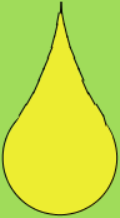
\includegraphics[height=30px]{water_warning}
	\end{center}
\end{minipage}
\begin{minipage}{0.85\textwidth}
	\textbf{Avertissement d'eau}\\
	Lorsqu'un bâtiment ne reçoit pas assez d'eau. Vous devez alors penser à ajouter des pompes à eau, ou bien, si des pompes à eau ne fonctionnent pas, à ajouter des centrales électriques.
\end{minipage}
\\
\\
\\
\begin{minipage}{0.1\textwidth}
	\begin{center}
		
\includegraphics[height=30px]{workforce_warning}
	\end{center}
\end{minipage}
\begin{minipage}{0.85\textwidth}
	\textbf{Avertissement d'emplois}\\
	Lorsqu'une entreprise a des emplois non pourvus de longue durée. Vous devez alors penser à agrandir vos zones résidentielles afin que de nouveaux habitants s'installent dans votre ville et aillent travailler.
\end{minipage}
\\
\\
\\
\begin{minipage}{0.1\textwidth}
	\begin{center}
		
\includegraphics[width=25px]{employement_warning}
	\end{center}
\end{minipage}
\begin{minipage}{0.85\textwidth}
	\textbf{Avertissement de chômage}\\
	Lorsqu'une maison a un résident au chômage de longue durée. Vous devez alors penser à ajouter des zones d'activités économiques afin que de nouvelles entreprises s'installent dans votre ville.
\end{minipage}
\\
\\
\\
\begin{minipage}{0.1\textwidth}
	\begin{center}
		
\includegraphics[width=30px]{taxes_warning}
	\end{center}
\end{minipage}
\begin{minipage}{0.85\textwidth}
	\textbf{Avertissement d'impôts}\\
	Lorsqu'une maison ou une entreprise paye plus d'impôts qu'elle ne le peut. Vous devez alors penser à diminuer les impôts pour le type de bâtiments concerné.
\end{minipage}



\section{Manipulation}

\subsection{Interface}
\begin{center}
	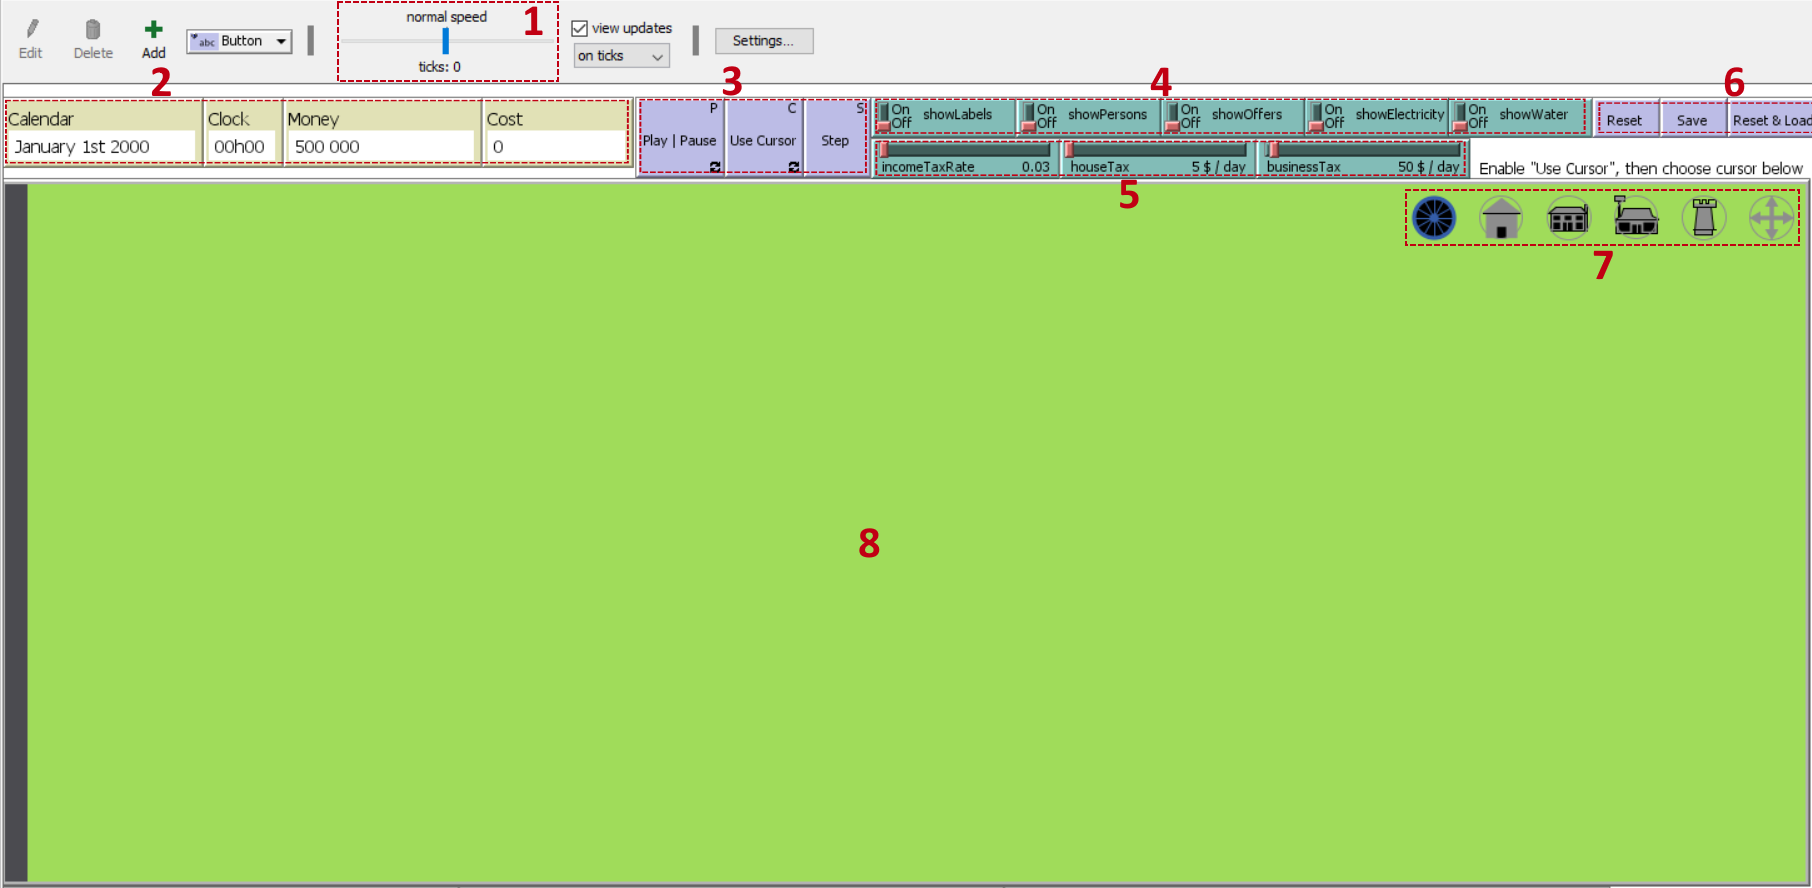
\includegraphics[width=\textwidth]{labeled_interface}
\end{center}

\subsubsection{1 : Vitesse de simulation}
Vous pouvez contrôler la vitesse de la simulation avec ce slider. La vitesse réelle d'exécution est limitée par la puissance de calcul de votre ordinateur et par le nombre d'informations à traiter dans la simulation. Pour améliorer les performances, pensez à désactiver le bouton ``Use Cursor'' lorsque vous ne l'utilisez pas.

\subsubsection{2 : Informations du jeu}
Vous pouvez voir les informations suivantes :
\begin{itemize}
	\item Calendrier : La date actuelle dans la simulation
	\item Horloge : L'heure actuelle dans la simulation
	\item Argent : L'argent que vous avez pour construire votre ville
	\item Coût : L'argent que vous allez dépenser si vous validez votre construction
\end{itemize}

\subsubsection{3 : Boutons du jeu}
Avec ces boutons et les raccourcis clavier associés vous pouvez :
\begin{itemize}
	\item Jouer et mettre en pause le jeu (touche P)
	\item Activer et désactiver l'utilisation des curseurs (touche C)
	\item Jouer un seul tick de jeu (touche S)
\end{itemize}

\subsubsection{4 : Visibilité des agents}
Avec ces switches vous pouvez afficher ou cacher les labels flottants des agents, les personnes, les offres d'emploi, l'électricité et l'eau.

\subsubsection{5 : Impôts}
Avec ces sliders vous pouvez contrôler le taux d'imposition sur le revenu, l'impôt sur les maisons et l'impôt sur les entreprises.

\subsubsection{6 : Boutons de la simulation}
Avec ces boutons vous pouvez :
\begin{itemize}
	\item Remettre à zéro la simulation et la ville
	\item Sauvegarder les structures (zones, centrales, pompes et routes) de la ville (écrase l'ancienne sauvegarde)
	\item Remettre à zéro la simulation et charger les structures de la sauvegarde
\end{itemize}
Pour sauvegarder et charger votre ville et non pas seulement les structures, il faut passer par le menu \textbf{File -> Export/Import -> Export/Import world}.

\subsubsection{7 : Curseurs}
Si le bouton ``Use cursor'' est activé alors vous pouvez avec votre souris sélectionner un des curseurs suivants :\\
\begin{itemize}
	\item
	\begin{minipage}{0.75\textwidth}
		\textbf{Route}\\
		Construisez une route en cliquant sur une route ou autoroute déjà existante et en glissant jusqu'à la position désirée
	\end{minipage}
	\begin{minipage}{0.2\textwidth}
		\begin{flushright}
			
\includegraphics[height=30px]{planners_road}
		\end{flushright}
	\end{minipage}
	
	\item
	\begin{minipage}{0.75\textwidth}
		\textbf{Zone résidentielle}\\
		Désignez une zone résidentielle en faisant un glisser déposer délimitant la zone souhaitée autour d'une route
	\end{minipage}
	\begin{minipage}{0.2\textwidth}
		\begin{flushright}
			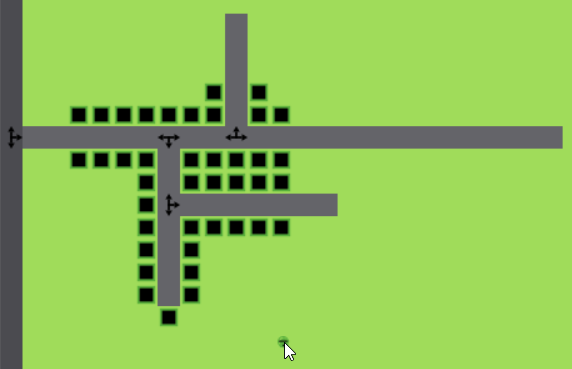
\includegraphics[height=55px]{planners_house_zone}
		\end{flushright}
	\end{minipage}
	
	\item
	\begin{minipage}{0.75\textwidth}
		\textbf{Zone d'activités économiques}\\
		Désignez une zone d'activités économiques en faisant un glisser déposer délimitant la zone souhaitée autour d'une route
	\end{minipage}
	\begin{minipage}{0.2\textwidth}
		\begin{flushright}
			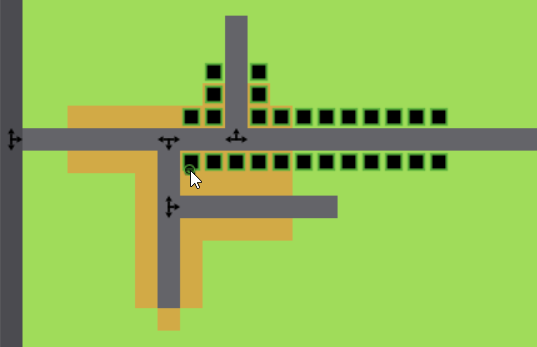
\includegraphics[height=55px]{planners_business_zone}
		\end{flushright}
	\end{minipage}
	
	\item \textbf{Centrale électrique}\\
	Construisez une ou des centrales électriques en cliquant ou en faisant un glisser déposer autour d'une route
	
	\item \textbf{Pompe à eau}\\
	Construisez une ou des pompes à eau en cliquant ou en faisant un glisser déposer autour d'une route
	
	\item
	\begin{minipage}{0.75\textwidth}
		\textbf{Intersections}\\
	Créez une intersection en cliquant sur un patch de route ou sélectionnez une intersection en cliquant sur celle-ci. Modifiez l'intersection sélectionnée en
	\end{minipage}
	\begin{minipage}{0.2\textwidth}
		\begin{flushright}
			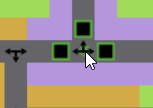
\includegraphics[height=55px]{intersection_edit}
		\end{flushright}
	\end{minipage}
	cliquant sur les directions à autoriser ou non. Validez en cliquant de nouveau sur l'intersection.
\end{itemize}

\subsubsection{8 : Votre ville}
Votre ville est entièrement vide au début du jeu sauf pour une autoroute qui longe le côté gauche de votre parcelle.
Vous pouvez interagir dans ce cadrant et observer votre ville évoluer.



\newpage
\subsection{Graphes}
Pour vous aider dans la gestion de votre ville, vous avez à votre disposition un ensemble de graphes qui vous apporterons des informations vous permettant de mieux prévoir vos actions ainsi que d'avoir une vue d'ensemble sur les différents aspects de votre ville.\\
Pour voir ces graphes, faites défiler l'interface vers le bas.
Tout les graphes représentent les informations sur une semaine glissante.
\begin{center}
	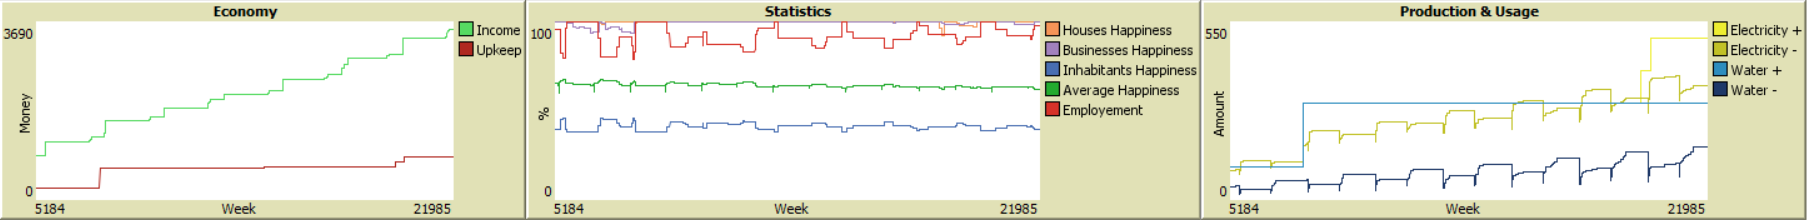
\includegraphics[width=\textwidth]{graphs}
\end{center}
\subsubsection{Graphe de l'économie}
Sur ce graphe vous pouvez facilement voir si vos coûts de maintenance dépassent vos revenus. Si c'est le cas c'est signe que vous avez essayé de développer votre ville trop rapidement. Pour remédier à cela, vous pouvez augmenter les différents impôts, mais le bonheur de votre ville en subira les conséquences.
\subsubsection{Graphe des statistiques}
Ces conséquences sont justement visibles sur ce deuxième graphe. Le bonheur global, de vos habitants, de vos maisons et de vos entreprises ainsi que le taux d'emploi sont affichés, vous permettant d'identifier la source d'un malheur. Si vous avez un taux d'emploi faible, c'est que vous devez essayer d'avoir plus d'entreprises dans votre ville.
\subsubsection{Graphe de production \& consommation}
Sur ce dernier graphe vous voyez apparaître la production et la consommation d'eau et d'électricité.
Cela vous permet de prévoir quand vous devrez ajouter une nouvelle centrale ou une nouvelle pompe à eau avant que votre ville ne manque de ressources.

\newpage
\subsection{Configuration}

\subsubsection{Configuration générale}
Dans le fichier \textbf{./config/config.txt} vous pouvez modifier les paramètres suivants :
\begin{itemize}
	\item Longueur d'une journée dans la simulation (en ticks)
	\item Heure où les offres d'emploi sont envoyées par les entreprises (en nombre de ticks après le début de la journée)
	\item Heure où les habitants quittent leur maison (en nombre de ticks après le début de la journée)
	\item Heure où les habitants rentrent chez eux (en nombre de ticks après le début de la journée)
	\item Heure où les habitants vont se coucher (en nombre de ticks après le début de la journée)
	\item Argent que vous avez au départ pour construire votre ville (en \$)
	\item Prix d'un morceau de route (en \$)
	\item Prix d'une centrale électrique (en \$)
	\item Prix d'une pompe à eau (en \$)
	\item Impôts sur les maisons (en \$/jour)
	\item Impôts sur les entreprises (en \$/jour)
	\item Taux d'imposition sur le revenu
	\item Coût de la maintenance d'un morceau de route (en \$/jour)
	\item Coût de la maintenance d'une centrale électrique (en \$/jour)
	\item Coût de la maintenance d'une pompe à eau (en \$/jour)
	\item Salaire de base d'un salarié (en \$/jour)
	\item Promotion cumulée maximum d'un salarié (en \$/jour)
	\item Vitesse de déplacement des offres d'emploi (en patch/tick)
	\item Vitesse de déplacement des véhicules (en patch/tick)
	\item Vitesse de déplacement des ressources (en patch/tick)
	\item Couleur de fond des labels (RGBA)
	\item Couleur du terrain vide (RGB)
	\item Couleur des autoroutes (RGB)
	\item Couleur des routes (RGB)
	\item Couleur des zones résidentielles (RGB)
	\item Couleur des zones d'activités économiques (RGB)
\end{itemize}

\newpage
\subsubsection{Autres configurations}
Dans le fichier \textbf{./config/gui.txt} vous pouvez modifier l'apparence et la position des curseurs.
Cela est utile si vous souhaitez modifier la taille de la simulation car les coordonnées dans le nouveau repère ne correspondront pas forcément à vos attentes.\\
Chaque ligne du fichier correspond à un curseur, chaque propriété du curseur est séparée par un espace. Ces propriétés sont, dans l'ordre :
\begin{itemize}
	\item Position x
	\item Position y
	\item Identifiant du curseur
	\item Nom de la forme de tortue du curseur
\end{itemize}
Dans le fichier \textbf{./config/highways.txt} vous pouvez modifier la position de l'autoroute et en ajouter d'autres.
Cela est utile dans le cas où vous souhaitez redimensionner la simulation mais également si vous souhaitez avoir plusieurs points d'entrée pour de nouveaux habitants dans votre simulation.\\
Chaque ligne du fichier correspond à une autoroute, chaque propriété de l'autoroute est séparée par un espace. Ces propriétés sont, dans l'ordre :
\begin{itemize}
	\item Position x du début de l'autoroute
	\item Position y du début de l'autoroute
	\item Position x de la fin de l'autoroute
	\item Position y de la fin de l'autoroute
\end{itemize}




\chapter{Simulations}
À chaque ajout d'une nouvelle fonctionnalité ou presque, j'ai refactoré une grande partie du code. Cela permet d'avoir un code et un résultat très cohérent dans son ensemble, mais rend impossible la comparaison d'une version à l'autre. Par exemple j'aurais aimé comparer le déplacement des agents sur les routes dans la première version et la version finale, mais le concept même de route n'est plus du tout le même dans sa structure et dans son exécution.\\
Il y a donc simplement une seule version pour laquelle je fais varier les situations initiales et/ou les paramètres pour évaluer les comportements. Toutes les simulations réalisées sont effectuées par rapport au temps et, sauf indication contraire, depuis le premier tick de la simulation jusqu'à un temps arbitraire suffisant permettant d'observer un phénomène.


\section{Resources}
\subsection{Consommation}
La consommation d'eau et d'électricité des maisons et des entreprises dépend du nombre de personnes utilisant les locaux. Pour observer cela on compare le nombre d'habitants à la maison et au travail à la consommation d'eau et d'électricité des maisons et des entreprises.
\begin{center}
	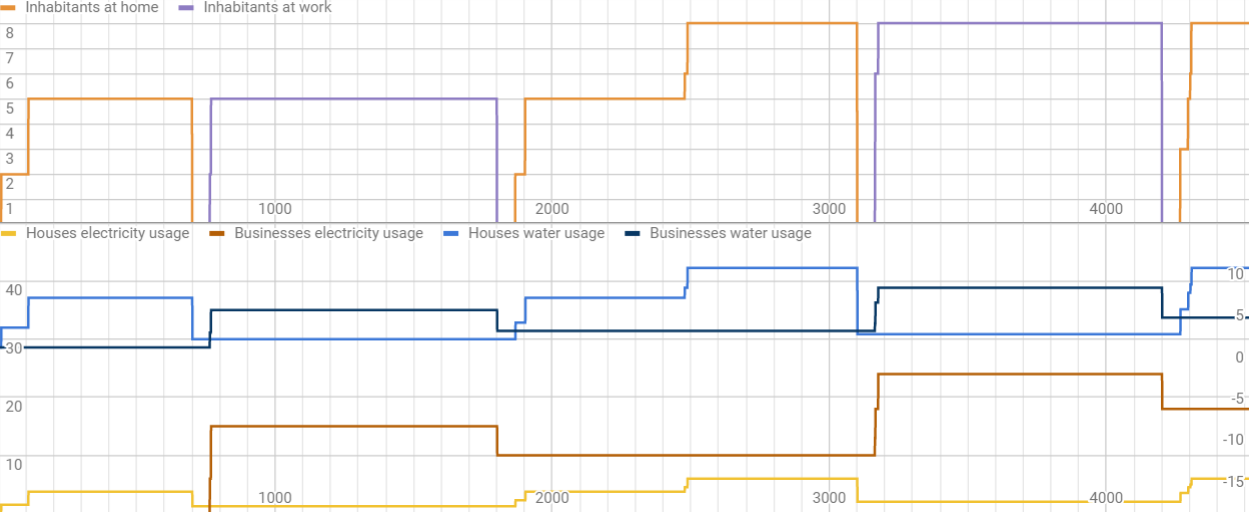
\includegraphics[width=\textwidth]{consumption}
\end{center}
On remarque bien qu'il y a une partie fixe de consommation même quand personne n'est présent. Cela est dû au fait que même quand il n'y a personne, les bâtiments utilisent un peu d'électricité. On voit bien qu'une partie de la consommation dépend du nombre de personnes présentes.

\subsection{Stockage}
En plus des maisons et entreprises, les pompes à eau consomment de l'électricité. Sans cette électricité, elles ne fourniraient pas d'eau.
Les bâtiments stockent plus de ressources qu'ils n’utilisent pour éviter qu'ils soient constamment en besoin d'une ressource. Leur capacité de stockage des ressources est toujours le double de leur consommation de la ressource.\\
L'électricité peut donc être soit sur les routes en déplacement, soit stockée dans les bâtiments. On souhaite observer l'évolution de l'électricité au cours du temps. On va donc placer une seule centrale électrique et aucun consommateur d'électricité. Puis on ajoute une pompe à eau (premier point rouge), puis on ajoute une deuxième pompe à eau, une zone résidentielle et une zone d'activités économiques (deuxième point rouge).
\begin{center}
	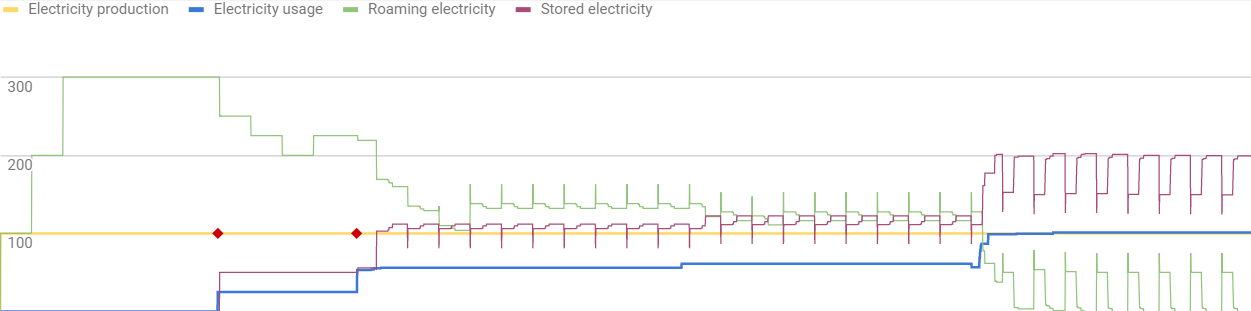
\includegraphics[width=\textwidth]{electricity_storage}
\end{center}
On peut voir que la production d'électricité est constante, c'est normal on n'ajoute pas de centrale.
On remarque que l'électricité sur les routes (courbe verte) augmente par palier 3 fois puis reste stable. Cela est dû au fait que l'électricité est produite toute les heures, et que les agents d'électricité disparaissent après 3 heures. Au bout de la 3ème heure donc, les nouveaux agents d'électricité remplacent les plus anciens.\\
Lorsqu'on ajoute la pompe à eau, on voit la consommation augmenter car elle utilise une partie de l'électricité. La pompe stocke également de l'électricité, ce qui se voit sur la courbe pourpre. Puisque la pompe absorbe des agents électriques, il y en a moins sur les routes.\\
Lorsqu'on ajoute la deuxième pompe à eau et les zones, on voit à nouveau la consommation et l'électricité stockée augmenter et l'électricité sur les routes diminuer. Petit à petit des maisons et entreprises s'installent dans les zones, et progressivement la consommation augmente.
Au bout d'un certain temps la consommation dépasse la production. On voit alors que l'électricité sur les routes commence à diminuer car elle n'est plus renouvelée à temps. La courbe verte n'est alors positive que pendant un court moment pendant que l'électricité se déplace de la centrale aux bâtiments.\\
Le graphe suivant montre la suite de la simulation.
\begin{center}
	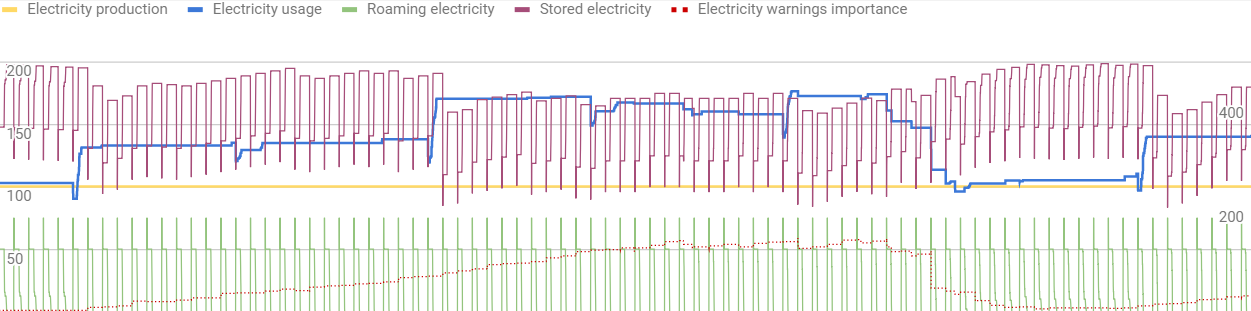
\includegraphics[width=\textwidth]{electricity_storage_2}
\end{center}
On remarque que des avertissements de manque d'électricité commencent à apparaître. Cela est dû au fait que bien qu'il y ait encore de l'électricité en stock dans certains bâtiments, les bâtiments les plus éloignés de la centrale électrique ne reçoivent jamais assez d'électricité.\\
La consommation augmente mais on remarque tout de même des petites descentes. Cela est dû aux maisons ou entreprises qui quittent la ville dû au manque d'électricité qui engendre du malheur.\\
Bien que la consommation augmente, l'électricité stockée elle diminue. Cela est dû au fait qu'il n'y a simplement pas assez d'électricité produite pour qu'elle soit stockée, et comme la consommation augmente, il y a moins d'électricité disponible pour être stockée.\\
Au bout d'un certain temps, la consommation descend brusquement, de même que les avertissements. Cela est signe que les maisons et entreprises ne supportaient plus le manque d'électricité et ont quittées la ville en masse..\\
Enfin on remarque une remontée de la consommation, suivi d'une remontée des avertissements, dû aux nouvelles maisons et entreprises qui s'installent. Un cycle stable commence.


\section{Bonheur}
\subsection{Attractivité}
L'attractivité de la ville influence la fréquence de nouveaux camions de déménagement. L'attractivité est basée sur le bonheur de la ville.
Pour vérifier que le nombre de camions varie proportionnellement en fonction du bonheur on observe le nombre de nouveaux camions avec un bonheur élevé, puis on augmente les taxes et supprime centrales électrique et les pompes à eau (point rouge sur le graphe) pour voir le changement de fréquence.
\begin{center}
	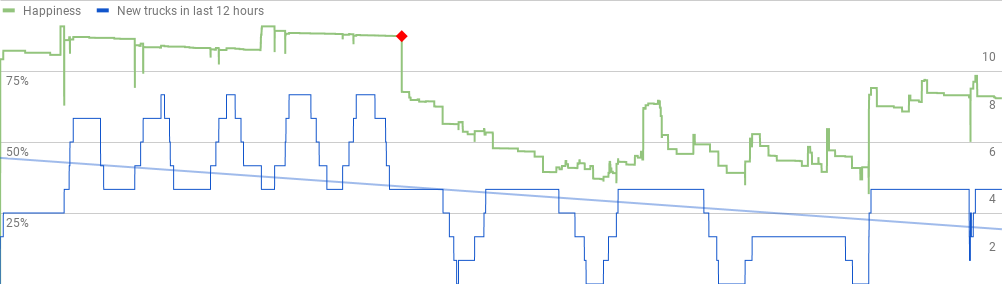
\includegraphics[width=\textwidth]{happiness_new_trucks}
\end{center}
On remarque en effet que lorsque le bonheur diminue, la fréquence de nouveaux camions aussi.\\
Il est intéressant de noter que le bonheur augmente après un certain temps sans toucher au système. Cela est dû au fait que toutes les personnes, maisons et entreprises malheureuses quittent la ville, ce qui fait remonter la moyenne de bonheur et donc la fréquence de nouveaux camions.


\newpage
\section{Revenu}
Le revenu est basé sur les impôts. Plus les impôts sont élevés, plus le revenu est grand. Mais si les impôts deviennent trop élevés et ne permettent pas aux habitants de survivre, ils quittent la ville.
On veut observer comment les différents impôts affectent le revenu. On compare donc le nombre d'employés, de maisons et d'entreprises avec le revenu obtenu.\\
On choisit 50\% comme taux d'imposition sur le salaire des employés, 50\$ comme impôt sur les maison et 100\% comme impôt sur les entreprises. Ces valeurs sont suffisamment grandes pour observer les changements sur le graphes tout en gardant la population suffisamment heureuse pour qu'elle ne parte pas.
\begin{center}
	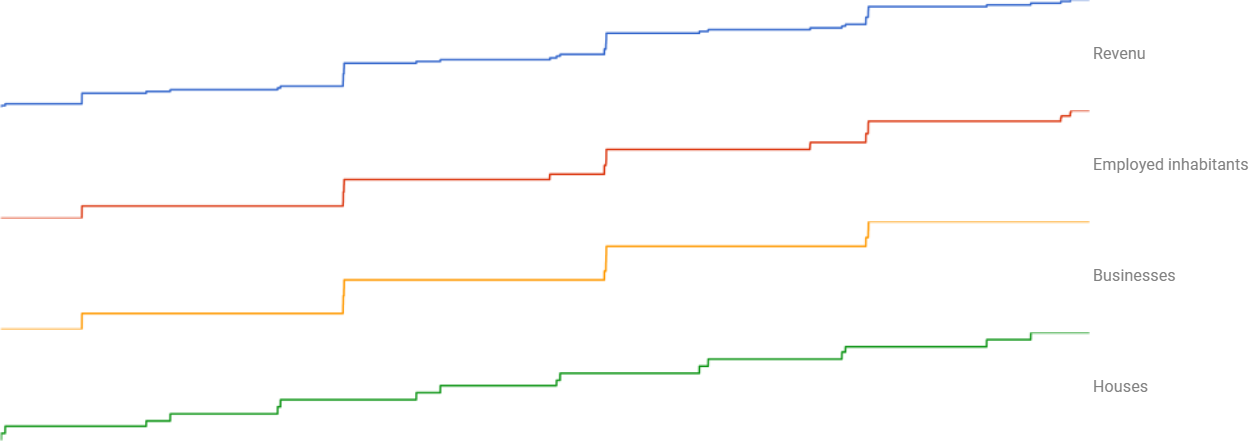
\includegraphics[width=\textwidth]{revenu}
\end{center}
On remarque en effet que chaque fois qu'il y a un nouvel employé, une nouvelle maison ou une nouvelle entreprise, le revenu augmente. On remarque également que le nombre d'entreprises augmente uniquement quand le nombre d'employés augmente. C'est parce que ces employés sont les créateurs de ces nouvelles entreprises. C'est également pour cela que la courbe forme un escalier régulier, car les habitants sortent de chez eux en même temps pour aller créer une entreprise.\\
Lorsque le nombre d'employés augmente mais pas le nombre d'entreprises, il s'agit de personnes recrutées via les offres d'emploi.


\newpage
\section{Impôts}
Les 3 types d'impôts affectent la ville de différentes manières. Pour observer leur impact ont prend une même ville et on lance la simulation avec des impôts différents.

\subsection{Maisons}
D'abord un impôt sur les maisons de 500\$ et 0 pour les autres. Avec un tel impôt, tous les habitants qui s'installent dans une maisons finiront par quitter la ville et détruire la maison.
\begin{center}
	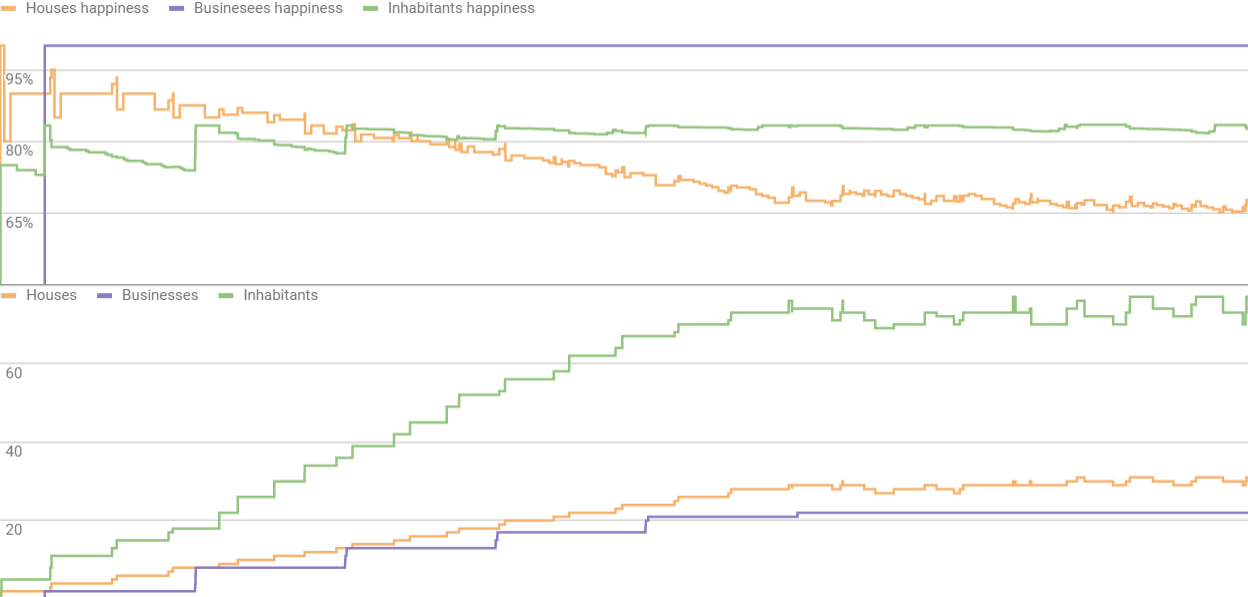
\includegraphics[width=\textwidth]{houses_taxes}
\end{center}
On remarque qu'il faut un certain temps pour que l'effet de l'impôt se fasse ressentir car si tout va bien pour une maison seul l'avertissement dû aux impôts rentre en compte dans le calcul du bonheur. Cet avertissement prend du temps à prendre de l'importance.\\
Le nombre de maisons et le bonheur des maisons atteint un équilibre après un certain temps. C'est parce que les premières maison qui s'étaient installées quittent enfin la ville sous la pression des impôts, et de nouvelles maisons viennent immédiatement les remplacer. Cela continue de manière cyclique ad vitam æternam.\\
On remarque que le nombre d'habitants est affecté de la même manière que le nombre de maisons, ce qui est logique car les habitants sont dans les maisons.

\newpage
\subsection{Entreprises}
Maintenant un impôt sur les entreprises de 1000\$ et 0 pour les autres. Avec un tel impôt, toutes les entreprises qui s'installent finiront par mettre la clé sous la porte.
\begin{center}
	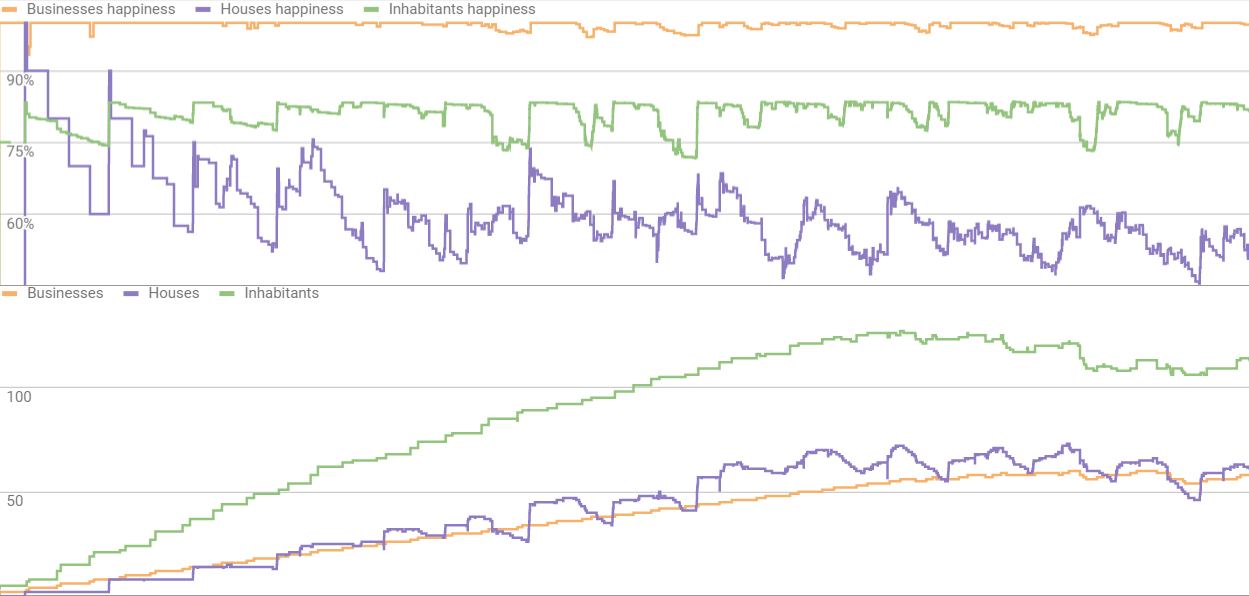
\includegraphics[width=\textwidth]{businesses_taxes}
\end{center}
On remarque que le bonheur des entreprises descend par paliers, en montant avant certains paliers. La montée est dû aux nouvelles entreprises qui s'installent et qui font remonter la moyenne avec un bonheur de 100\%. Les paliers sont dû au fait que les avertissements augmentent en importance au même moment. Les paliers disparaissent peu à peu car des entreprises disparaissent aléatoirement et d'autres les remplacent.\\
Après un certain temps, il y a autant d'entreprises qui installent que d'entreprises qui quittent la ville, ce qui provoque un équilibre du nombre d'entreprises observée.
On remarque que le nombre de maisons et par conséquent le nombre d'habitants est affecté par cet équilibre. Cela est dû au fait qu'il n'y a pas assez d'entreprises pour satisfaire suffisamment les habitants qui quittent donc la ville.

\newpage
\subsection{Habitants}
Enfin un impôt de 0\$ pour les maisons et les entreprises, et un impôt sur le salaire des habitants de 0\% d'abord, 50\% au premier point rouge et 75\% au 2ème point rouge.
\begin{center}
	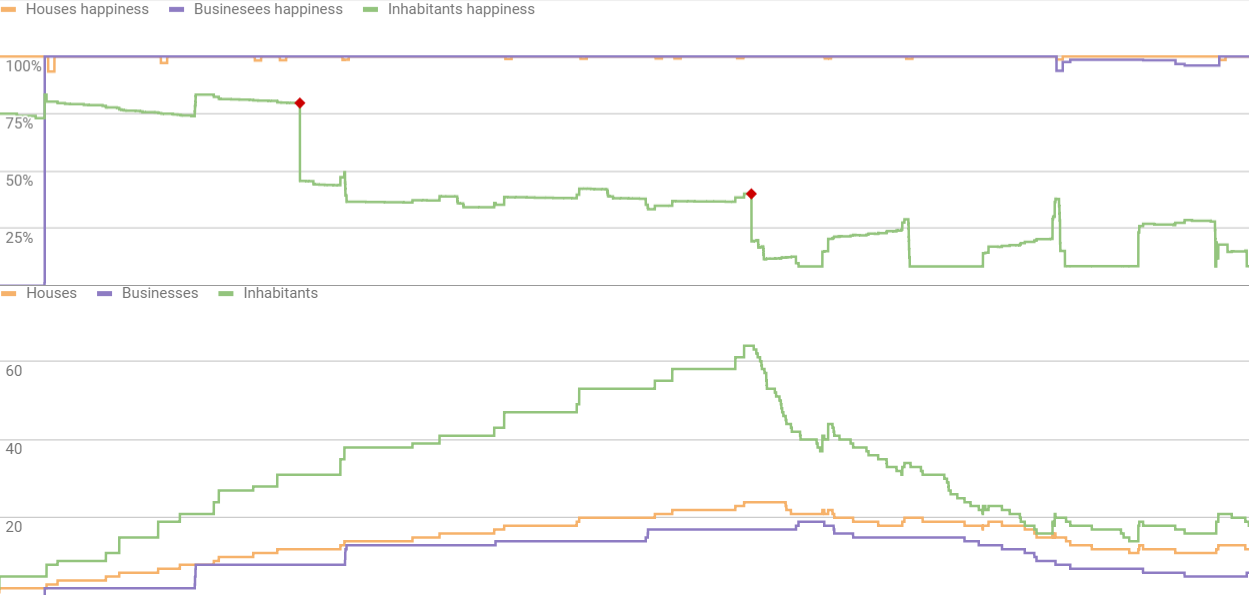
\includegraphics[width=\textwidth]{inhabitants_taxes}
\end{center}
On remarque que le bonheur est affecté par le changement du taux d'imposition de 0\% à 50\% mais la croissance de la population n'est pas affectée. Cela est dû au fait que le salaire de base couvre les besoins des habitants même taxés à 50\%, ils n'ont donc pas de raison de vouloir quitter la ville.\\
Après 75\% cependant, tous les habitants se retrouvent dans l'incapacité de survire et quittent la ville, faisant chuter la population. Lorsque tous les habitants d'une maison l'ont quitté, la maison est détruite, c'est pourquoi on observe une diminution du nombre de maison en parallèle. Comme il n'y a plus de personnes pour travailler, les entreprises mettent la clé sous la porte, ce qui explique la diminution de leur nombre.\\
Les sauts de bonheur qu'on peut apercevoir sont dû aux nouveaux habitants rejoignant la ville, qui n'ont pas encore de travail et sont donc heureux car au chômage seulement depuis peu.



\chapter*{Conclusion}
\addcontentsline{toc}{chapter}{Conclusion}
Compte tenu de l'énorme quantité de valeurs paramétrables et de l'infinité de situations provoquées par le joueur, les analyses ne sont pas exhaustives. Il est donc encouragé d'aller jouer soi-même avec la simulation et d'essayer de modifier les paramètres dans le fichier de configuration pour observer les changements induits.
\end{document}